\section{PŘESNÝ DIFERENCIÁLNÍ STUPEŇ (MOS/bipolar, odporová zátěž, aktivní zátěž)}
Analýza, pravidla přesného návrhu, ekvivalentní vstupní ofset, proudová nesymetrie transkonduktačního diferenčního stupně, výstupní napěťová nesymetrie zesilovače a jejich vztahy

Pro dif. stupeň s bipolárem je přklad uveden v kapitole 5.4. Na to lze navázat výpočet aktivní MOS zátěže v kapitole 6.1.

\subsection{Diferenční MOS stupeň s odporovou/MOS aktivní zátěží}
Mějme požadavek, že $\sigma$\textsubscript{vos} musí být menší než nějaké napětí (řádově jednotky mV).

PMOS diferenciální stupeň navrhneme jako proloženou dvojici PMOS tranzistorů s šířkou W =2*L. Hledáme takovou délku, aby výsledný $\sigma$\textsubscript{vos} byl menší, než námi chtěný vč. rezervy, tzn $\sigma$\textsubscript{vos hledaný} < $\sigma$\textsubscript{vos}. Hledáme v tabulce:
\begin{figure}[h]
   \begin{center}
     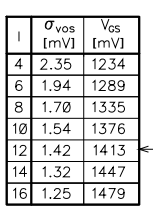
\includegraphics[scale=0.6]{images/tab.png}
   \end{center}
   \caption{Tabulka pro určení $\sigma$\textsubscript{vos}}
\end{figure}

\begin{figure}[h]
   \begin{center}
     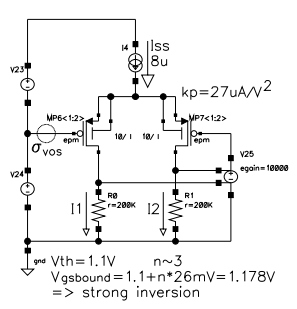
\includegraphics[scale=0.6]{images/PMOS.png}
   \end{center}
   \caption{Diferenciální PMOS}
\end{figure}

Tento nesouběh $\sigma$\textsubscript{vos} se dá přenést na nesouběh $\sigma$\textsubscript{i} proudu pomocí transkonduktace gm:
\begin{equation}
gm=\sqrt{I_{ss}*kp*\frac{W}{L}}
\end{equation}
\begin{equation}
\sigma_{i}=\sigma_{vos}*gm
\end{equation}

\subsubsection{Aktivní MOS zátěž}
Pokud má být chyba $\sigma$\textsubscript{ion}, která přísluší aktivní zátěži zanedbatelná, musí být menší, než polovina chyby $\sigma$\textsubscript{i}:
\begin{equation}
\sigma_{Ion} < \frac{\sigma_{i}}{2}
\end{equation}

Aktivní zátěž navrhneme opět jako proloženou dvojici NMOS tranzistoru s šířkou W, kde úkolem je najít délku L, kdy chyba $\sigma$\textsubscript{ion} této aktivní zátěže bude rovna nebo menší $\sigma$\textsubscript{ion hledaná} < $\sigma$\textsubscript{ion}. 
\begin{figure}[h]
   \begin{center}
     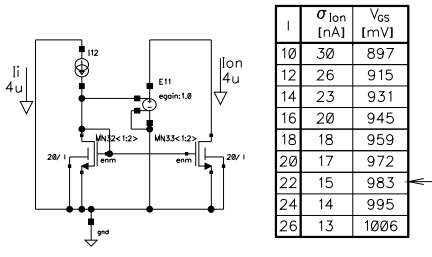
\includegraphics[scale=0.6]{images/akt.png}
   \end{center}
   \caption{Aktivní NMOS zátěž}
\end{figure}

Výsledná chyba $\sigma$\textsubscript{ion} je:
\begin{equation}
\sigma_{ion}=\sqrt{\sigma_{i}^2+\sigma(ion)^2}
\end{equation}

Z ní pak lze přepočítat chybu napěťové nesymetrie $\sigma$\textsubscript{vos}:
\begin{equation}
\sigma_{vos}=\frac{\sigma_{Io}}{gm}
\end{equation}

\subsection{Výstupní napěťová nesymetrie zesilovače a jejich vztahy}
Výstupní offset zesilovače závisí na vstupním offsetu tohoto zesilovače (viz. kapitola 8). Jeho eliminace je zde také popsána vč. vztahů.






